\documentclass{article}

% Language setting
% Replace `english' with e.g. `spanish' to change the document language
\usepackage[english]{babel}
\usepackage{changepage}
% Set page size and margins
% Replace `letterpaper' with `a4paper' for UK/EU standard size
\usepackage[letterpaper,top=2cm,bottom=2cm,left=3cm,right=3cm,marginparwidth=1.75cm]{geometry}

% Useful packages
\usepackage{amsmath}
\usepackage{graphicx}
\usepackage[colorlinks=true, allcolors=blue]{hyperref}
\setlength{\parindent}{2em}

\title{Merlin Bridge WhitePaper}
\author{Eason.Z \\dev@merlinprotocol.org \and Rilke \and shier \and Hannah}
\date{DRAFT Version 0.1.2}

\begin{document}
\maketitle

\begin{center}
\Large\textbf{A Remarkable Ruse}
\end{center}

\begin{abstract}
With the rapid development of cryptocurrency, Bitcoin and Ethereum have emerged as the two largest ecosystems in the industry. Bitcoin, as the pioneer blockchain application, is often referred to as "digital gold," holding a significant position in the cryptocurrency market due to its security and value storage characteristics. On the other hand, Ethereum serves as a versatile blockchain technology platform, offering extensive possibilities for the development of smart contracts and decentralized applications (DApps).
\par As blockchain technology continues to advance, the demand for cross-chain integration from Bitcoin to Ethereum has been steadily increasing. As of March 2022, approximately \$21.8 billion worth of assets have been locked in cross-chain protocols, with Wrapped Bitcoin (WBTC) \cite{wbtc}accounting for over 50\% of this total. However, more than 90\% of the bridges facilitating cross-chain asset transfers utilize a centralized custody approach. In May 2023, the Multichain cross-chain protocol declared an abrupt cessation of operations, resulting in the inability to transfer locked assets valued at \$1.26 billion within its system.
\par Merlin Bridge stands as a leading decentralized and trustless protocol-level solution for Bitcoin cross-chain interoperability. This solution enables anyone to provide cross-chain channel services to users through the protocol, earning corresponding service fees. Importantly, the protocol is entirely decentralized and trustless, allowing users to engage in cross-chain operations without relying on third parties.Within Merlin Bridge, the protocol's governance is based on a Decentralized Autonomous Organization (DAO) model, facilitating a more community-driven and democratic decision-making mechanism. This signifies that community members can collectively participate in the management and governance of the protocol, ensuring that its development and optimization align with the overall interests.
\end{abstract}

\section{Addressing These Issues Through Cross-Chain Channels}
\begin{adjustwidth}{4em}{4em}"Storing Bitcoin with a commercial custody provider or distributing it across many decentralized nodes— which approach do you think is safer?"
\end{adjustwidth}
\par Currently, the Bitcoin custody business holds a considerable market share within the industry. Many compliant institutions are offering custody services to users while continually updating and upgrading security technologies. However, no one can guarantee with absolute certainty that events like the "Mt. Gox Bitcoin theft" won't happen again. If a large-scale custodial institution encounters security issues, it could not only impact related operations but also potentially disrupt the entire Web3 industry.(Refer to the "Mt. Gox" incident).
\par By dispersing users' stored Bitcoin across numerous nodes, the safety of the entire system's assets remains intact even if certain nodes encounter security issues, thereby achieving high fault tolerance. Based on this concept, we've designed cross-chain service channels. This channel shares similarities with the Lightning Network's\cite{ln} micropayment\cite{bitcoinjmicropay} channels, featuring attributes such as channel capacity and asset collateral. Simultaneously, we also aspire for Merlin Bridge to play a proactive role in expanding the Bitcoin ecosystem, akin to the Lightning Network.
\par The core function of cross-chain channels is to receive Bitcoin locked within the cross-chain bridge. The creators of these channels engage in overcollateralization of other assets on the Ethereum network to ensure the security of the held Bitcoin. In case of malicious behavior within cross-chain channels, safety for Bitcoin assets is maintained through auction-based liquidation of channel collateral assets.

\section{Key Challenges}
\begin{enumerate}
    \item How is the security of the locked Bitcoin ensured within the protocol?
    \item How to ensure that there is no additional issuance of MBTC when Bitcoin enters the Ethereum network?
    \item How is the assurance provided that users will definitely receive their extracted Bitcoin after MBTC destruction?
\end{enumerate}

\section{Knowledge}
\subsection{Merlin Bitcoin(MBTC)}
\par Bitcoin bridge in Ethereum as ERC-20 standard tokens, pegged 1:1 to Bitcoin.
\subsection{Struct of Block}
\subsubsection{Bitcoin's Block}
\begin{figure}[h]
    \centering
    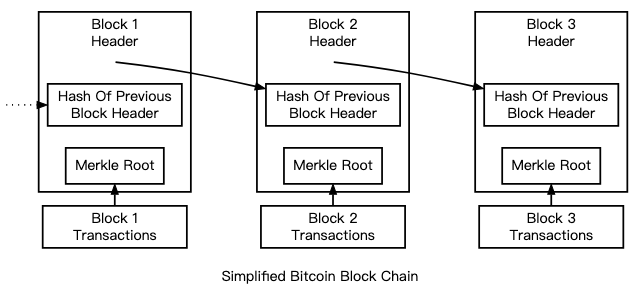
\includegraphics[width=0.85\textwidth]{bitcoin_block.png}
    \caption{\label{fig:bitcoin_block}Simplified Bitcoin Block.}
    \label{fig:bitcoin_block}
\end{figure}
The illustration above shows a simplified version of a block chain\cite{nakamoto}. A block of one or more new transactions is collected into the transaction data part of a block. Copies of each transaction are hashed, and the hashes are then paired, hashed, paired again, and hashed again until a single hash remains, the merkle root of a merkle tree.
\par The merkle root is stored in the block header. Each block also stores the hash of the previous block’s header, chaining the blocks together. This ensures a transaction cannot be modified without modifying the block that records it and all following blocks.
\subsubsection{Ethereum's Block}
\begin{figure}[h]
\centering
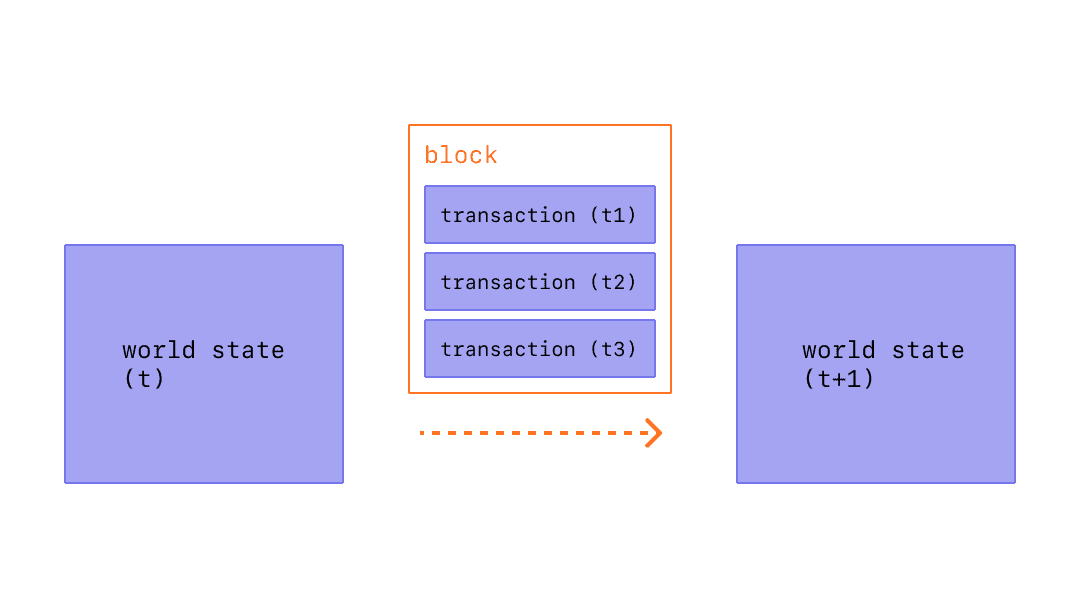
\includegraphics[width=1\textwidth]{eth_block.png}
\caption{\label{fig:eth_block}Simplified Ethereum Block.}
\end{figure}
To preserve the transaction history, blocks are strictly ordered (every new block created contains a reference to its parent block), and transactions within blocks are strictly ordered as well. Except in rare cases, at any given time, all participants on the network are in agreement on the exact number and history of blocks, and are working to batch the current live transaction requests into the next block. \cite{ethpaper}
\subsection{UTXO and Account}
\subsubsection{Unspent Transaction Output (UTXO)}
The figure above shows the main parts of a Bitcoin transaction. Each transaction has at least one input and one output. Each input spends the satoshis paid to a previous output. Each output then waits as an Unspent Transaction Output (UTXO) until a later input spends it. When your Bitcoin wallet tells you that you have a 10,000 satoshi balance, it really means that you have 10,000 satoshis waiting in one or more UTXOs.
\begin{figure}[h]
\centering
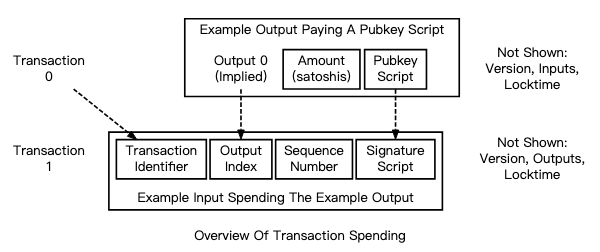
\includegraphics[width=1\textwidth]{utxo.png}
\caption{\label{fig:utxo}Overview of Transaction Spending.}
\end{figure}
\par When a transaction is completed, any unspent outputs are recorded into a database as inputs that can be used later for a new transaction.
\subsubsection{Account}
An Ethereum account is an entity with an ether (ETH) balance that can send transactions on Ethereum. Accounts can be user-controlled or deployed as smart contracts.\\
Ethereum has two account types:
\begin{itemize}
    \item Externally-owned account (EOA) – controlled by anyone with the private keys
    \item Contract account – a smart contract deployed to the network, controlled by code. Learn about smart contracts
\end{itemize}
\begin{figure}[h]
\centering
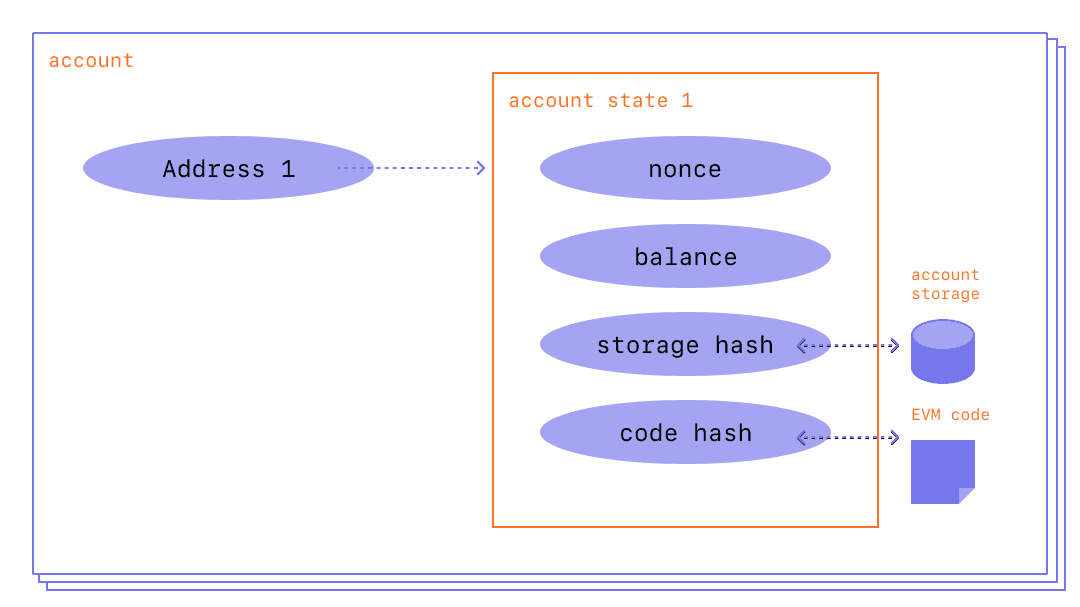
\includegraphics[width=1\textwidth]{account.png}
\caption{\label{fig:account}Overview of Ethereum Account.}
\end{figure}
Ethereum accounts have four fields:
\begin{itemize}
    \item nonce – A counter that indicates the number of transactions sent from an externally-owned account or the number of contracts created by a contract account. Only one transaction with a given nonce can be executed for each account, protecting against replay attacks where signed transactions are repeatedly broadcast and re-executed.
    \item balance – The number of wei owned by this address. Wei is a denomination of ETH and there are 1e+18 wei per ETH.
    \item codeHash – This hash refers to the code of an account on the Ethereum virtual machine (EVM). Contract accounts have code fragments programmed in that can perform different operations. This EVM code gets executed if the account gets a message call. It cannot be changed, unlike the other account fields. All such code fragments are contained in the state database under their corresponding hashes for later retrieval. This hash value is known as a codeHash. For externally owned accounts, the codeHash field is the hash of an empty string.
    \item storageRoot – Sometimes known as a storage hash. A 256-bit hash of the root node of a Merkle Patricia trie that encodes the storage contents of the account (a mapping between 256-bit integer values), encoded into the trie as a mapping from the Keccak 256-bit hash of the 256-bit integer keys to the RLP-encoded 256-bit integer values. This trie encodes the hash of the storage contents of this account, and is empty by default.
\end{itemize}

\subsection{Smart Contract and Signature Script}
\subsubsection{Signature Script}
The Bitcoin signature script is a stack-based scripting language used to verify inputs and outputs in Bitcoin transactions. It ensures that only valid transactions can be added to the blockchain, thus maintaining the security and integrity of Bitcoin. The Bitcoin signature script consists of a series of operation codes (OP\_Codes) and data items, presented in bytecode form. In a transaction, the input script and output script are attached to the input and output, respectively, to verify the legitimacy of the transaction.\cite{wikicontracts}
Here are several common types of signature scripts:
\begin{itemize}
    \item Pay-to-Public-Key-Hash (P2PKH): P2PKH is the most common Bitcoin signature script type. In P2PKH transactions, the output script contains the recipient's public key hash. To unlock this transaction output, the sender must provide a signature corresponding to the public key and the original public key itself. This signature script is typically represented as "OP\_DUP OP\_HASH160 <PubKeyHash> OP\_EQUALVERIFY OP\_CHECKSIG."
    \item Pay-to-Script-Hash (P2SH): P2SH is a signature script type used for multi-signature and more complex scripts. In P2SH transactions, the output script contains a script hash, corresponding to the recipient's script. The sender must provide an unlocking script matching the recipient's script to unlock the output. This signature script is typically represented as "OP\_HASH160 <ScriptHash> OP\_EQUAL."
    \item Pay-to-Witness-Public-Key-Hash (P2WPKH): P2WPKH is a form of Segregated Witness (SegWit). In P2WPKH transactions, the output script contains the recipient's public key hash, and the unlocking script directly includes the signature corresponding to the public key. This signature script is typically represented as "<Signature> <PublicKey>."
    \item Pay-to-Witness-Script-Hash (P2WSH): P2WSH is another form of SegWit used to support multi-signature and other complex scripts. In P2WSH transactions, the output script contains a script hash, and the unlocking script contains data matching the recipient's script. This signature script is typically represented as "0 <ScriptHash>."
\end{itemize}
\subsubsection{The Smart Contract}
A "smart contract" is simply a program that runs on the Ethereum blockchain. It's a collection of code (its functions) and data (its state) that resides at a specific address on the Ethereum blockchain.
\par Smart contracts are a type of Ethereum account. This means they have a balance and can be the target of transactions. However they're not controlled by a user, instead they are deployed to the network and run as programmed. User accounts can then interact with a smart contract by submitting transactions that execute a function defined on the smart contract. Smart contracts can define rules, like a regular contract, and automatically enforce them via the code. Smart contracts cannot be deleted by default, and interactions with them are irreversible.
\subsection{Oracle}
In smart contracts, an oracle is a mechanism used to bring external data into the blockchain, enabling smart contracts to interact with real-world information. Since smart contracts themselves cannot directly access external data, oracles serve as a bridge connecting the blockchain and the real world, providing inputs of external data to smart contracts.\cite{oralce}\\
Within smart contracts, oracles can serve various purposes, such as:
\begin{itemize}
    \item Providing Price Data: Smart contracts can utilize oracles to access real-world price data for executing conditions and triggering contract operations, such as options contracts, insurance contracts, and more.
    \item External Event Triggering: Oracles can be employed to introduce external events (like weather, sports match results, etc.) into smart contracts and trigger corresponding contract logic.
    \item Cross-Chain Interaction: In cross-chain interactions, oracles can be utilized to retrieve data from other blockchain networks, facilitating interoperability between different blockchains.
\end{itemize}
\subsection{SPV(Simplified Payment Verification)}
It is possible to verify payments without running a full network node. A user only needs to keep a copy of the block headers of the longest proof-of-work chain, which he can get by querying network nodes until he's convinced he has the longest chain, and obtain the Merkle branch linking the transaction to the block it's timestamped in. He can't check the transaction for himself, but by linking it to a place in the chain, he can see that a network node has accepted it, and blocks added after it further confirm the network has accepted it.\cite{spv}
\begin{figure}[h]
\centering
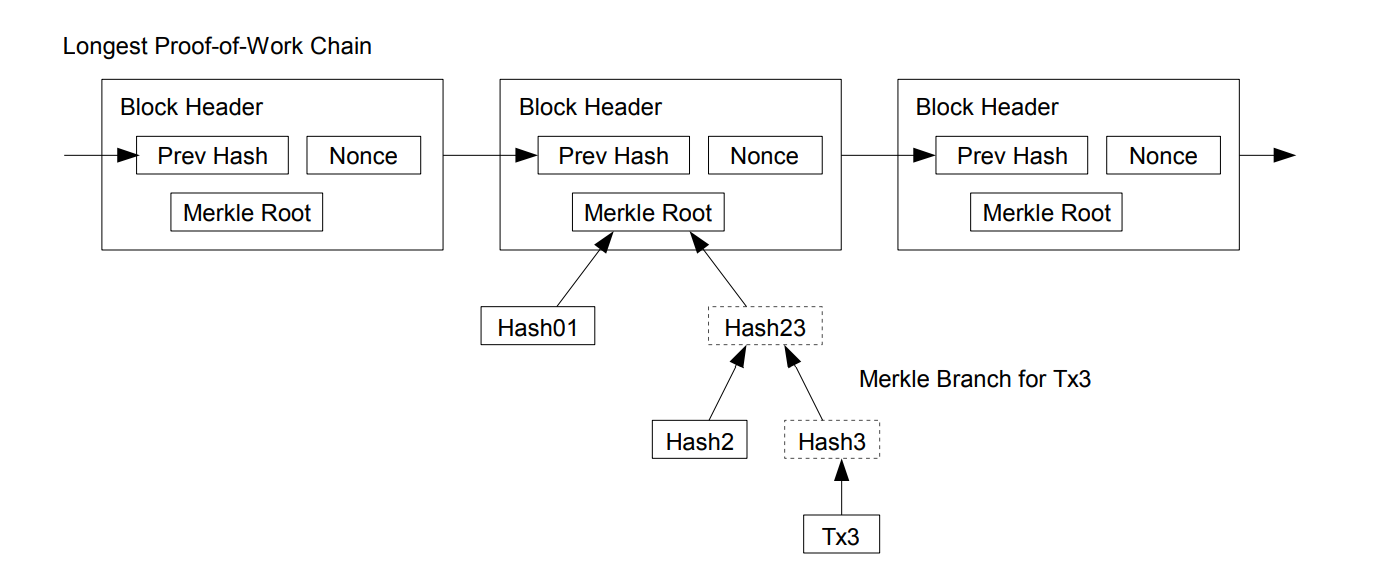
\includegraphics[width=1\textwidth]{spv.png}
\caption{\label{fig:spv}Overview of Simplified Payment Verification.}
\end{figure}
\par As such, the verification is reliable as long as honest nodes control the network, but is more vulnerable if the network is overpowered by an attacker. While network nodes can verify transactions for themselves, the simplified method can be fooled by an attacker's fabricated transactions for as long as the attacker can continue to overpower the network. One strategy to protect against this would be to accept alerts from network nodes when they detect an invalid block, prompting the user's software to download the full block and alerted transactions to confirm the inconsistency. Businesses that receive frequent payments will probably still want to run their own nodes for more independent security and quicker verification.
\subsection{Bitcoin Atomic Swap}
Atomic swaps use Hashed Time Lock Contracts (HTLCs), a type of smart contract, to facilitate a trustless exchange of digital assets\cite{lamportclocks}. Smart contracts employ an automated process that self-executes once all predetermined conditions encoded within the contract are met.\\
Bitcoin atomic swaps are possible thanks to two key components encoded in Bitcoin’s HTLCs:
\begin{enumerate}
    \item Hashlock. A hashlock is a cryptographically hidden key generated by the person that initiated a transaction. This key ensures that swaps are only finalized once both parties approve the transaction.
    \item Timelock. Timelocks are created as a Check-Lock-Time-Verify command (CLTV) or Check Sequence Verify (CSV). With CLTV, funds within a transaction are locked or released based on date and time. With CSV, funds are locked or released after a certain number of blocks are generated. In simpler terms, timelocks set a deadline for swaps. If both parties do not approve of the swap before a set time, the timelock acts as a safety mechanism and voids the transaction. In this situation, funds will be sent back to their respective owners.
\end{enumerate}
\section{Architecture}
\subsection{Roles and Responsibilities}
\subsubsection{Developer Community}
\par The developer community is an integral part of the Merlin Protocol ecosystem, responsible for project development and innovation. In the early stages, it is led by the Merlin Foundation and receives funding support. The developer community is committed to building a series of blockchain infrastructure smart contracts that serve the Bridge. Their work ensures the smooth operation and continuous development of the Merlin Protocol.\\
Responsibilities include:
\begin{itemize}
    \item On-chain data monitoring system, responsible for monitoring cross-chain service provider transaction activities.
    \item Off-chain smart contract triggers.
    \item Liquidation system.
\end{itemize}
\subsubsection{Cross-Chain Channel Service Providers}
Merlin Bridge welcomes anyone to become a Cross-Chain Channel Service Provider, contributing to the smooth operation of Merlin Bridge. The corresponding Cross-Chain Channel Service Providers can earn up to 1.5\% of transaction fees (subject to future community governance through voting).
\begin{figure}[h]
\centering
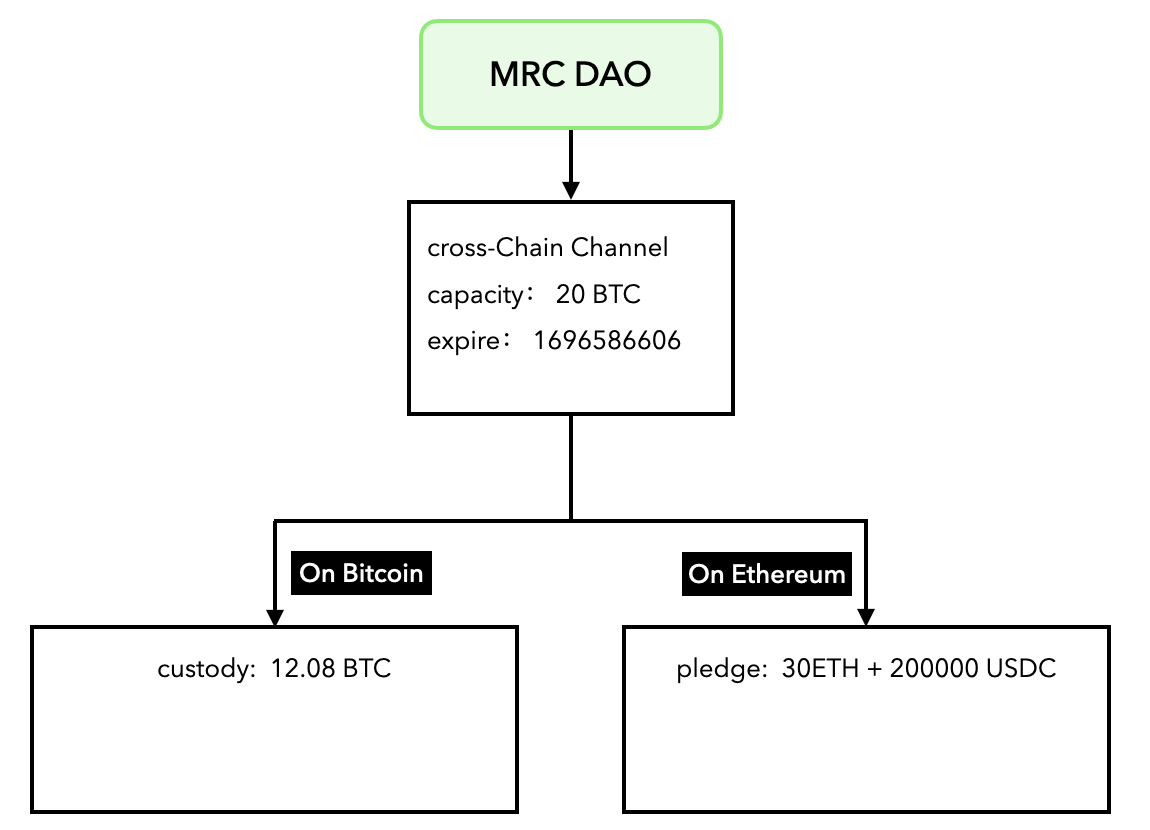
\includegraphics[width=1\textwidth]{services.png}
\caption{\label{fig:services}Accounts with Cross-chain Channel.}
\end{figure}
\par A Cross-Chain Channel encompasses two accounts: one on the Bitcoin network and the other as an Ethereum account. The Bitcoin public key is used to receive assets that users deposit in the channel, while the channel service provider maintains the channel capacity by over-collateralizing assets on the Ethereum account. This over-collateralization effectively secures the Bitcoin assets.\\
Process:
\begin{enumerate}
    \item Submit an application to the developer community and provide a public key for Bitcoin locking (the custodial address provided is not used on the Bitcoin network to reduce the burden on oracles). After approval from the developer community, registration for Bitcoin network query services will be added to the oracle contract.
    \item Once the Bitcoin receiving address is generated, it's added to the oracle's SPV service, becoming a data source for smart contract programming.
    \item The service provider determines the channel capacity for the Cross-Chain Channel service and pledges 150\% worth of USDC and ETH as collateral to ensure the security of the Bitcoin funds.
    \item Merlin Bridge gateway display.
\end{enumerate}
\par Please note that the provided translation is a literal representation of the information. Depending on the context, the wording might need to be adjusted for clarity and coherence.
\subsubsection{Oracle Cluster}
An oracle cluster is a system composed of an Ethereum smart contract and an off-chain server cluster, designed to bring transaction data from specific addresses in the Bitcoin network onto the blockchain. Its primary function is to inform smart contracts about changes in balance for monitored addresses in the Bitcoin network. Through the oracle cluster, smart contracts can obtain real-time updates from the Bitcoin network, enabling them to execute corresponding logic and operations.
\subsubsection{Liquidators}
Liquidators refer to users participating in the liquidation auctions of the Merlin Bridge. They can utilize Bitcoin to purchase unstable debt, acquire collateral assets, and engage in the auction process. The involvement of liquidators is crucial for maintaining the stability of MBTC, as they ensure the liquidation of collateral from Cross-Chain Channel Service Providers through the auction mechanism, thereby mitigating the risk of malicious behavior by the channel service providers.
\subsubsection{Customer}
Converting Bitcoin to MBTC allows it to be made available within Ethereum smart contracts and participate in various activities within the Ethereum ecosystem.
\subsection{Implementation}
\subsubsection{Model}
Cross-Chain Channels:\\
\par Cross-Chain Service Nodes are executable programs running on servers that are responsible for handling business logic, interacting with smart contracts, and communicating with web3 wallets.
Key attributes of nodes:
\begin{itemize}
    \item Channel States: Unactivated, Activated, Expired, Frozen, Paused, Closed.
    \item Channel Capacity: Each node has a predetermined capacity for the cross-chain channel, which represents the maximum amount of Bitcoin it can host. This capacity is established before the node is activated, ensuring a stable cross-chain asset processing capability throughout its operation.
    \item Minimum Channel Capacity: Similar to micro-payment channels, there's a minimum capacity limit set for the channel to ensure service quality and stability.
    % \item Channel Expiry: Each cross-chain channel has an expiration period during which it can provide cross-chain services to users. After expiration, the channel needs to be reactivated, and collateral assets and hosted Bitcoins are settled to ensure the security of cross-chain assets. This mechanism guarantees the stable operation of cross-chain services and reliable asset transfers.
\end{itemize}
Channel Gateway:\\
\par Merlin Bridge is composed of numerous cross-chain channels, and users need to select a suitable channel through the network before conducting cross-chain operations. Channel ranking supports sorting by capacity limit, available amount, and total cross-chain asset amount, making it convenient for users to choose according to their needs.
\\Public Channels:\\
\par In the early stages of ecosystem development, to ensure the smooth operation of channels and provide users with high-quality cross-chain services, the foundation will be responsible for building and maintaining public cross-chain channels. When other channels experience anomalies that lead to the need for Bitcoin liquidation, these Bitcoins will be held in the public channel. It is anticipated that within the next two years, as the number of channels grows, the foundation will gradually close the public channels.
\subsubsection{Implementing bitcoin cross-chain transfers to the Ethereum network}
The difficulty in cross-chain transfers lies in ensuring consistency of transaction states across the two chains, including transaction order, token quantities, and handling transaction rollbacks in case of failures.、、
Simplified Process:
\begin{enumerate}
    \item Users initiate a transaction on the Bitcoin network to transfer Bitcoin into a cross-chain channel.
    \item The cross-chain channel synchronizes Bitcoin transaction data and converts the corresponding Bitcoin from the account into MBTC.
\end{enumerate}
\par The simplest approach involves storing complete Bitcoin transaction data within a smart contract, but this is evidently impractical. However, relevant transaction data can be stored outside the Ethereum smart contract and queried through an oracle for the necessary transaction data. In theory, this allows internal validation of Bitcoin transactions' validity within the smart contract, ensuring that MBTC is not minted when Bitcoin enters the Ethereum network.
\par In this context, we employ Simplified Payment Verification (SPV) to validate the validity of Bitcoin transactions, with data sourced from an oracle and verification algorithms implemented within the smart contract.
\begin{figure}[h]
\centering
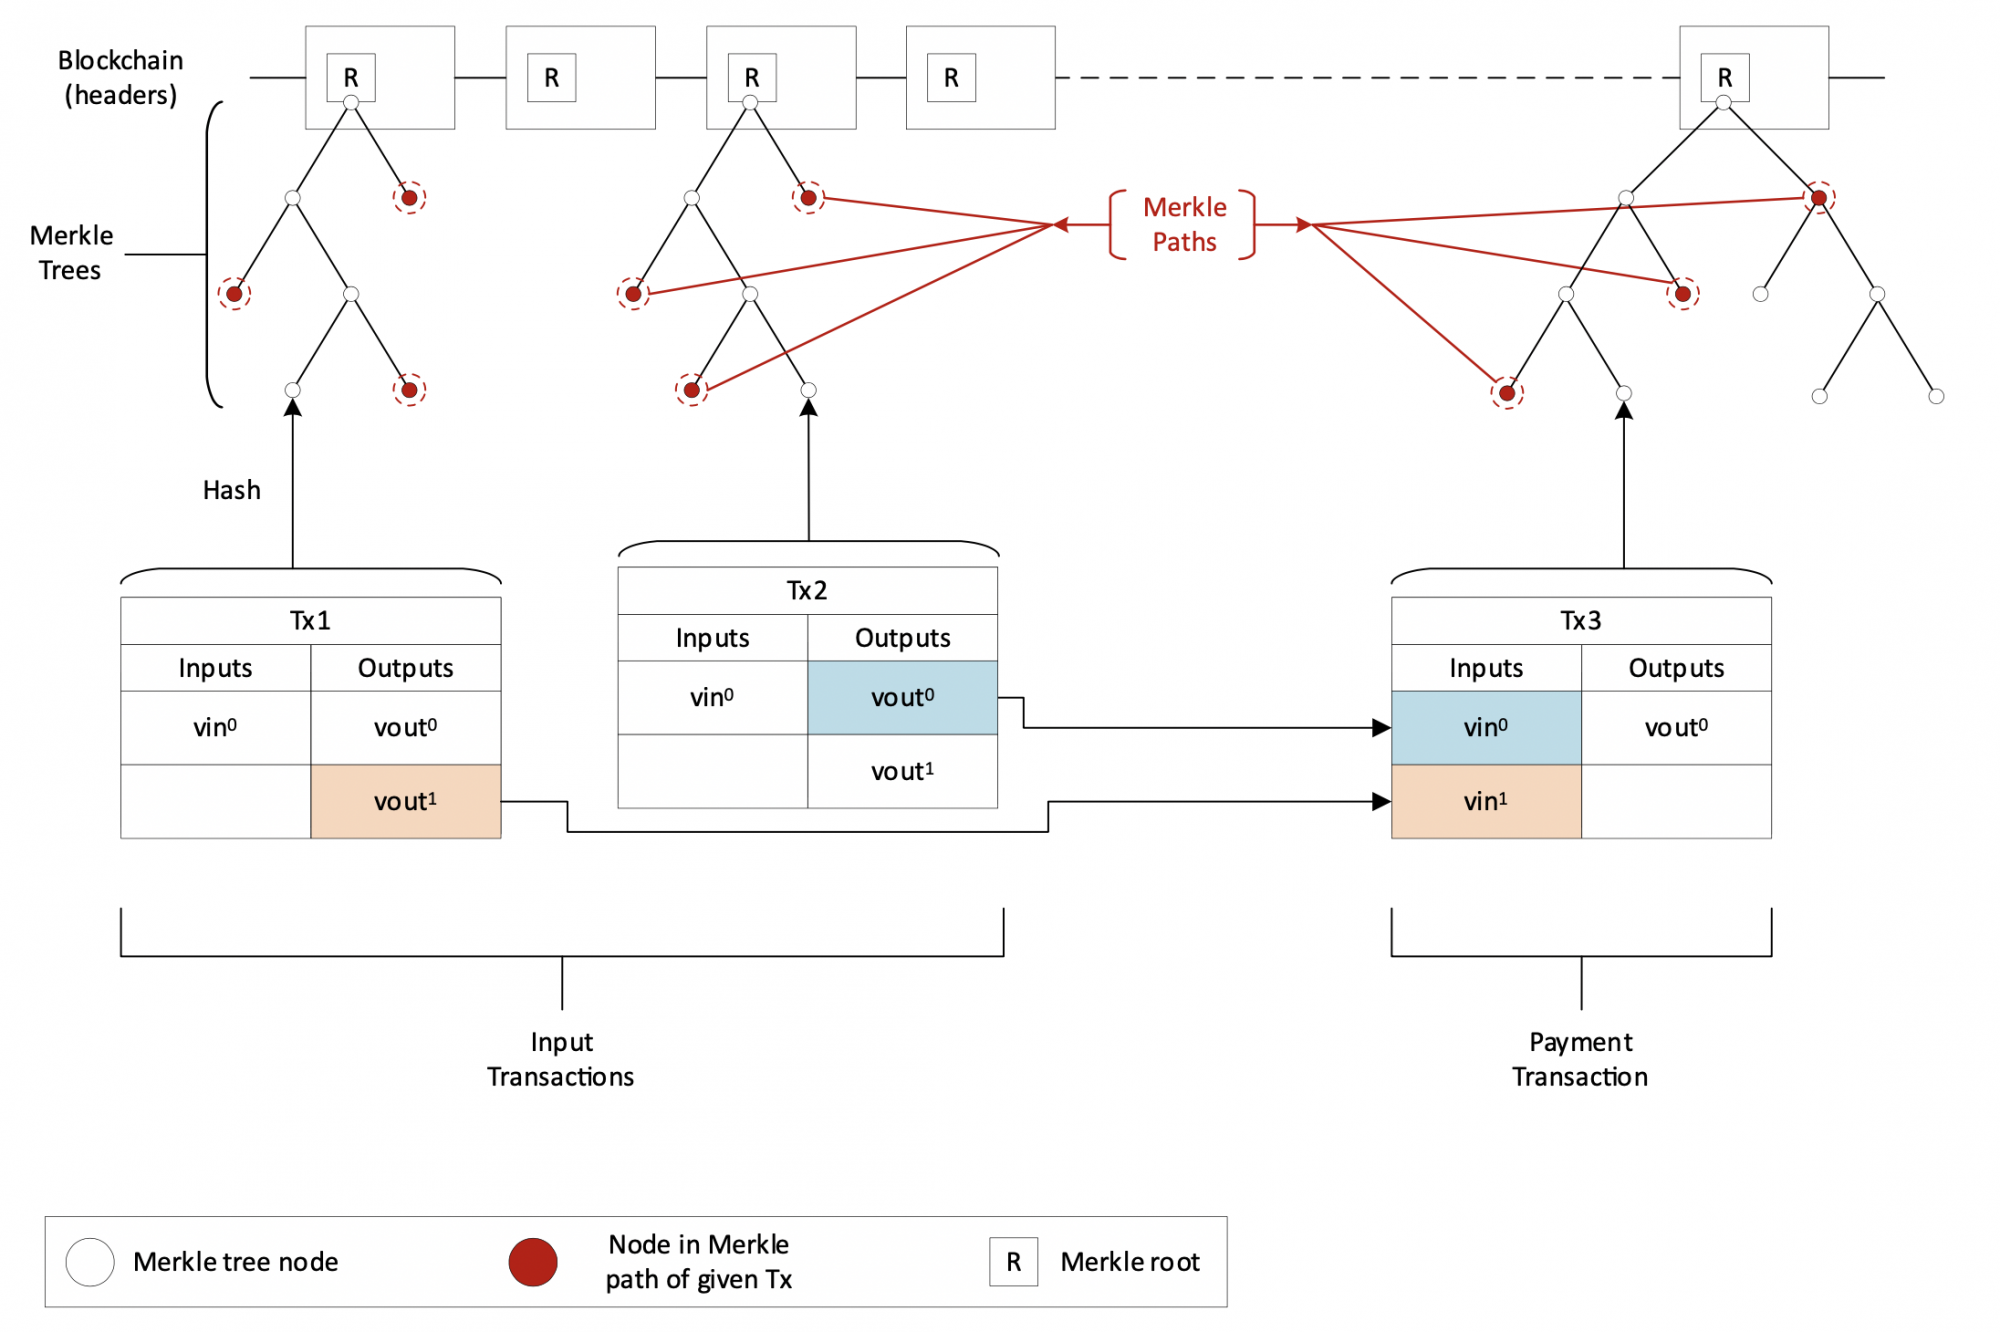
\includegraphics[width=0.85\textwidth]{spv2.png}
\caption{\label{fig:spv2}Verification.}
\end{figure}
\par Bitcoin transactions consist of inputs and outputs, where inputs essentially refer to the outputs of previous transactions. To verify the existence of a transaction, 1+n Merkle computations are required:
\begin{enumerate}
    \item Merkle path of the Bridge-in transaction hash, querying whether the block header exists in the oracle.
    \item Merkle paths of n inputs in the Bridge-in transaction, querying whether the block headers exist in the oracle.
\end{enumerate}
\par The corresponding Merkle paths are provided by the business system and passed into the smart contract as an array. In Solidity, Merkle computation is supported and widely used in various fields, such as NFT whitelist settings. The next step is to address the issue of oracle data storage.
\par For the oracle to provide SPV query services to the contract, it needs to store all Bitcoin block hashes. Each Bitcoin block header is 80 bytes, and currently, all headers collectively occupy around 60MB of storage. To alleviate the oracle's burden, the protocol will choose a specific height to provide SPV query services, estimated to be at height 750,000. Prior to this height, Merkle root hashes won't be queryable in the oracle. Within the cross-chain channel, certain business protective measures will be taken, requiring users to perform a consolidation transaction first to ensure that input transactions occur after the service height. Only then can they enter the cross-chain channel. Although this might cause some inconvenience, it significantly enhances system stability.
\par The smart contract can already determine whether a transaction exists on the Bitcoin network via the oracle. The next crucial step is to resolve the transaction details, mainly verifying whether output scripts conform to protocol standards.
\par The average size of a Bitcoin transaction is around 250 bytes. The transaction size is unrelated to the transfer amount but rather depends on the number of inputs and outputs. As the number of inputs and outputs increases, Bitcoin transactions inflate. To reduce the data flow into the smart contract, the protocol dictates that Bridge-in transaction inputs cannot exceed 3, and outputs cannot exceed 2. These limitations effectively control transaction size, ensure the contract's normal operation, and maintain network efficiency and security.
\par To further distinguish the channel bridge-in transactions, the protocol has expanded the spending script of outputs (referring to Ordinals) and embedded certain fundamental cross-chain information within the script. This information is used for the distribution of MBTC tokens when parsing Bitcoin transaction scripts within the cross-chain channel. The script content is as follows:
\begin{verbatim}
OP_FALSE
OP_IF
  OP_PUSH "Merlin/v/1.0"
  OP_PUSH 1
  OP_PUSH "bridge-in"
  OP_PUSH 0
  OP_PUSH "des=eth&channel=0xalice&account=0xbob"
OP_ENDIF
\end{verbatim}
\par The protocol content is written in plaintext into the output spending script, including the protocol version number, operation type, and parameters.
\par The OP\_FALSE OP\_IF ... OP\_ENDIF within the script is used to encapsulate a certain amount of data. It's important to note that these scripts are essentially no-operations; they do not alter the semantics of the scripts containing them. Ultimately, these scripts will be appended to the specifics of spending Bitcoin UTXOs (Unspent Transaction Outputs).
\par The Treasury smart contract for MBTC on the Ethereum chain will handle the minting and burning of MBTC tokens on the Ethereum network, following this process:
\begin{enumerate}
    \item Users initiate a bridge-in transaction and write it onto the blockchain.
    \item The oracle updates block header data to ensure synchronization of MBTC status with the Bitcoin network.
    \item The contract invokes the Mint function of the MBTC Treasury to mint the corresponding amount of MBTC tokens for the user.
    \item Transaction Validity Verification:
        \begin{enumerate}
            \item Cross-chain channel and capacity validity verification.
            \item Bridge-in transaction identification.
            \item MBTC minting.
        \end{enumerate}
\end{enumerate}
\par The contract allows any Ethereum account to trigger the MBTC minting functionality without permission restrictions. We have now achieved a 1:1 minting of Bitcoin on the Ethereum network.
\subsubsection{Destruction of MBTC on the Ethereum Network and Redemption on the Bitcoin Mainnet}
Cross-Chain Channel Service Providers have control over users' custodied Bitcoin, thus potential malicious motives exist. To ensure the smooth operation of cross-chain channels and the security of user assets, we employ a mechanism similar to FileCoin's over-collateralization and penalties for malicious behavior to constrain channel conduct.
\begin{itemize}
    \item Cross-chain channels require a 150\% asset collateral as a deposit.
    \item Users receive a 1.5\% fee when performing Bitcoin redemptions in the Bridge-out process.
\end{itemize}
Process:
\begin{itemize}
    \item Users initiate a Bitcoin redemption transaction through the MBTC Treasury contract. The contract destroys the corresponding MBTC, records the Bitcoin receiving address, and the channel information used.
    \item The cross-chain channel instantly captures the contract-initiated transaction, parses the data, and initiates a Bitcoin transfer of the corresponding amount to the user.
    \item The oracle captures this Bitcoin transaction and records its data on the blockchain.
    \item The cross-chain channel service successfully completes the transaction and closes the channel.
\end{itemize}
\subsection{Pledging and Liquidation}
Price Feeding by Oracles is utilized to provide prices for different assets, including BTC, ETH, and on-chain assets that are being used for collateral. Different channels compute the value of minted MBTC against the total collateral value. This step doesn't require real-time on-chain computation and can be presented on a frontend page.
\par Real-time calculation of the MBTC liabilities and collateral ratios for each channel. When the total collateral ratio falls below 120\%, liquidators can partially liquidate assets of that node to maintain the collateral ratio. When the collateral ratio drops below 110\%, the foundation will liquidate all collateral assets.
\par Liquidators (other channel nodes, whitelisted liquidators, foundation members) can initiate partial liquidation transactions. By paying any amount of BTC to the public channel, they can apply to liquidate collateral assets of any node. The contract will attempt to proportionally deduct collateral assets worth 105\% of the paid BTC and pay it to the liquidator. However, the condition for the partial liquidation transaction to be effective is that after calculating the collateralized BTC and the corresponding value of collateral being liquidated, the total collateral ratio drops below 120\%\cite{aavev3}.Calculation:
\begin{itemize}
    \item Assuming the current collateral ratio has dropped to 116\%, let's take an example of MBTC worth a total value of \$400 and collateral assets worth \$465. In this case, the maximum potentially liquidated assets would be 25\% of the total assets, i.e., liquidating \$100 worth of MBTC and \$105 worth of collateral assets. The remaining assets would be MBTC worth a total value of \$300 and collateral assets worth \$360. This would restore the collateral ratio to 120\%, resulting in a loss of only \$5 for the node. This loss represents a relatively low proportion of around 1.1\% relative to the total collateral assets, indicating a relatively low risk exposure.
    \item After liquidation, the node's liability for accepting BTC would decrease by \$100, and the public channel's liability for accepting BTC would increase by \$100. Subsequent BTC acceptance would be primarily handled by the public channel.
    \item When liquidators conduct liquidation, they can also issue MBTC themselves and use the freely issued MBTC to pay the under-collateralized node for the liquidation transaction. The node being liquidated would be obliged to pay the corresponding amount of collateral assets in exchange for MBTC. When nodes fulfill their acceptance obligations, they can use the MBTC from other nodes they hold for the acceptance process.
\end{itemize}
\par The initial collateral ratio is set at 150\%. This not only prevents immediate liquidation in the event of a certain decrease in asset value but also ensures a higher fund utilization and asset yield, maintaining a balance between safety and returns.
\par Based on recent data, the correlation coefficient between BTC and ETH returns is 87\%. This high asset correlation ensures the stability of the collateral ratio in the case of significant market fluctuations. The volatility of ETH returns is 1.25 times that of BTC (the actual value being 1.1). Combined with the initial 150\% collateral ratio and a portfolio composition of 65\% ETH and 35\% USD, the overall collateral asset composition against Bitcoin's price volatility is calculated as 1.5 * 65\% * 1.25 = 1.22. This portfolio setting naturally maintains the collateral ratio above 120\%.
\par Suppose a node issues a total of \$100 worth of MBTC, requiring \$97.5 of ETH and \$52.5 of USDC as collateral assets:
\begin{enumerate}
    \item In the case of a moderate BTC price increase of, say, 40\%, resulting in the issuance of \$140 worth of MBTC. Based on historical data, with an expected ETH price increase of 50\%, the total value of the collateral asset composition is \$97.5 * 1.5 + \$52.5 = \$196.25, resulting in a collateral ratio of 140\%, which is sufficiently safe.
    \item In the scenario of a significant BTC price increase of 200\%, issuing \$300 worth of MBTC, with an expected ETH price increase of 250\%, the total value of the collateral asset composition becomes \$97.5 * 3.5 + \$52.5 = \$388.75, resulting in a collateral ratio of 130\%, still within a safe margin.
    \item Regardless of the magnitude of BTC's increase, this asset composition setting ensures that the expected collateral ratio doesn't fall below 1.22.
    \item In the case of a slight BTC price decrease of 40\%, resulting in the issuance of \$60 worth of MBTC. Based on historical data, with an expected ETH price decrease of 50\%, the total value of the collateral asset composition becomes \$97.5 * 0.5 + \$52.5 = \$100, resulting in a collateral ratio of 166\%. Asset depreciation would even lead to a higher total collateral ratio.
\end{enumerate}
\subsection{Ghost Bitcoin}
\par Ghost Bitcoin refers to a special type of transaction provided by cross-chain service channels that allows for the issuance of MBTC without the need for actual Bitcoin. Ghost Bitcoin transactions require the issuance and destruction of MBTC to be completed within a single block, along with the payment of corresponding transaction fees.
\par When there is arbitrage potential in MBTC transactions on the Ethereum network, users can swiftly engage in liquidity arbitrage through Ghost Bitcoin transactions, without any capital requirement. Ghost Bitcoin is a unique technical feature of MBTC. Leveraging Ghost Bitcoin, MBTC will gain enhanced market liquidity.
\section{Incentives}
Merlin Protocol, as an open ecosystem protocol, will utilize the MRC token to incentivize meaningful actions within the ecosystem during its early development stages. This will drive the flourishing growth of the ecosystem.
\subsection{Token Rights}
\begin{enumerate}
    \item Voting Rights: Merlin Protocol is a decentralized on-chain protocol, and during the process of protocol upgrades and adjustments to core parameters, MRC token holders play the role of co-builders of the protocol and participate in the protocol's public governance.
    \item Earnings Rights: MRC token holders can stake MRC tokens within the protocol to capture the results of participating in investments related to Real-World Assets (RWA). Earnings include both MRC tokens and crypto stablecoins.
    \item Usage Rights: As a cryptographic asset with intrinsic value support, MRC tokens possess certain usage rights.
        \begin{enumerate}
            \item When becoming a cross-chain channel service provider, MRC tokens can be used as collateral for a certain percentage.
            \item Used in investments related to RWAs.
        \end{enumerate}
\end{enumerate}
\subsection{Merlin Protocol Governance}
Merlin Protocol is a decentralized on-chain protocol, and during the process of protocol upgrades and adjustments to core parameters, MRC token holders are considered co-builders of the protocol and participate in its public governance.
\begin{adjustwidth}{4em}{4em}
1 MRC Token = 1 Vote
\end{adjustwidth}
There are two types of voting governance:
\begin{enumerate}
    \item Regular Voting: Wallet addresses holding 1 million MRC or more have a 7-day voting period during each regular upgrade. A vote with over 50\% approval is considered passed.
    \item Emergency Voting: In cases of urgent issues requiring a vote for protocol upgrade, the Merlin Protocol Foundation or the development team's wallet addresses need only 30\% circulating MRC support to execute the upgrade.
\end{enumerate}
\section{Prospects and Impact}
\par In the early stages of the ecosystem, the assets pledged for the channels primarily consist of stablecoins such as ETH, USDT, and USDC. As the development stages progress, we will open community proposals to expand the list of pledged assets. This approach helps improve the circulation of MBTC generated by the protocol within other ecosystems, thus fostering mutual growth.
\par Furthermore, as the amount of Bitcoin locked in the Merlin Bridge increases, the governance token MRC will also gain more liquidity. Under objective conditions, we will initiate community voting to consider including MRC as part of the assets eligible for channel pledging. This step enhances the overall utility and value of the ecosystem.
\subsection{Outlook for Future Development}
\par The Ethereum ecosystem has entered the era of Layer2 solutions. In the future, more Layer2 public chains will emerge, all requiring high-quality assets to support their ecosystems and creating significant market opportunities. After completing the Ethereum cross-chain functionality of Merlin Bridge, we will move forward to support Layer2 networks. Users will be able to seamlessly move in and out of Layer2 networks through our protocol, participating in a broader range of financial activities. This expansion into the Layer2 space signifies our commitment to providing users with more opportunities and access to a growing ecosystem.
\bibliographystyle{plain}
\bibliography{references}
\end{document}